\begin{recipe}{Coffee with a Chemex\textsuperscript{\texttrademark} Coffee Maker}{3 servings}{10 minutes}
\ing[?]{c.}{water, boiled}
Place filter in Chemex\textsuperscript{\texttrademark} coffee maker.  Pour about half of a cup of hot water (around \unit[200\0]{F}) through the filter, and dump water in sink.  The point of this is to warm and clean the filter, and make it adhere more readily to the glass.
\ing[?]{c.}{coffee, coarsely ground}
Add coffee grounds to filter.  Pour about half of a cup of hot water gently over the grounds.  Watch the grounds ``bloom,'' during which, if the beans are fresh, the coffee grounds will expand and bubble.  Only use enough water to moisten the grounds.
\newstep
Slowly fill Chemex\textsuperscript{\texttrademark} coffee maker with hot water (around \unit[200\0]{F}) and let strain.  When finished straining, refill with hot water, and strain again.  It may be necessary to reheat the water for second batch of straining.
\newstep
Transfer coffee to carafe or thermos.
\end{recipe}
\begin{figure}[b!]
\begin{center}
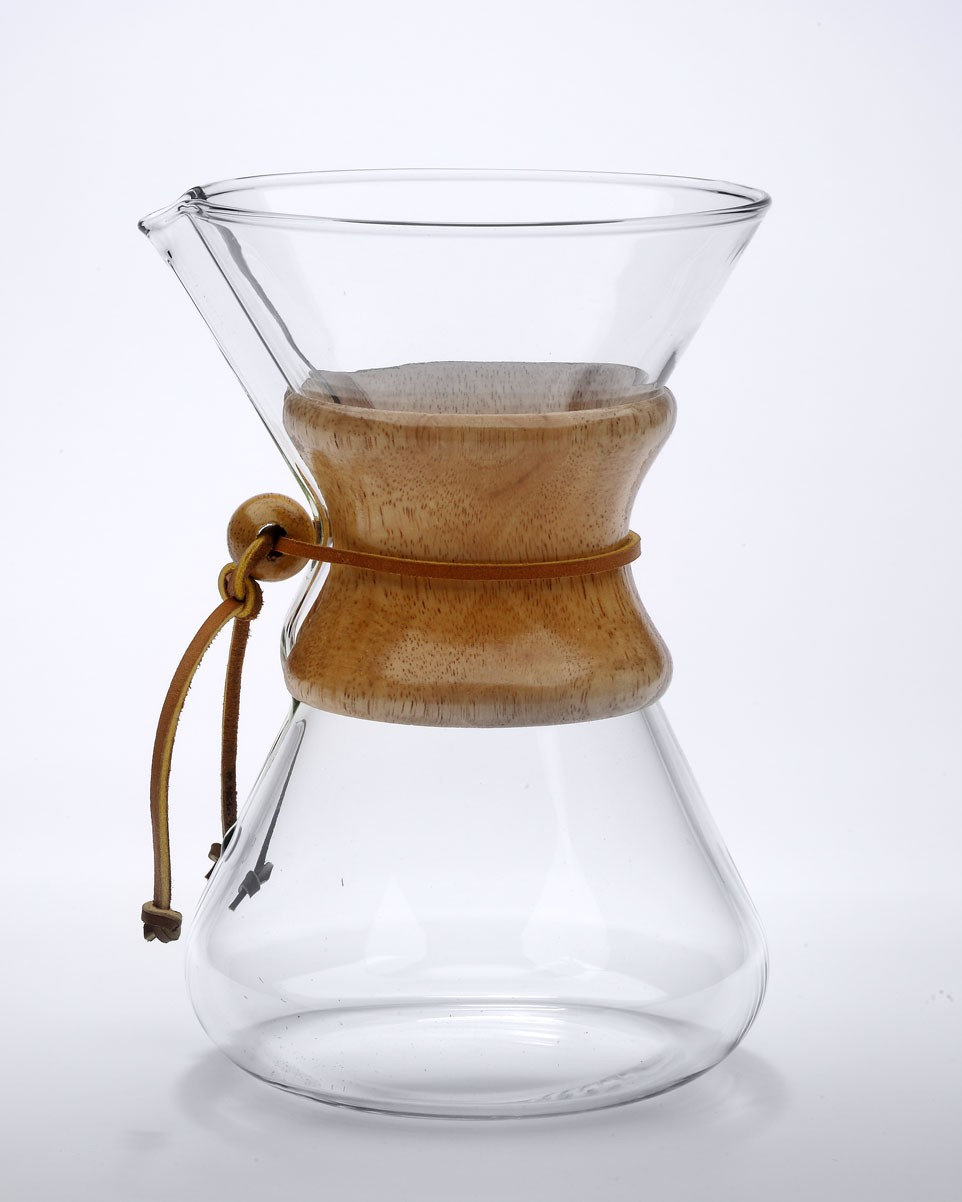
\includegraphics[height=0.32\textwidth]{./figures/chemex}
\hspace{0.1\textwidth}
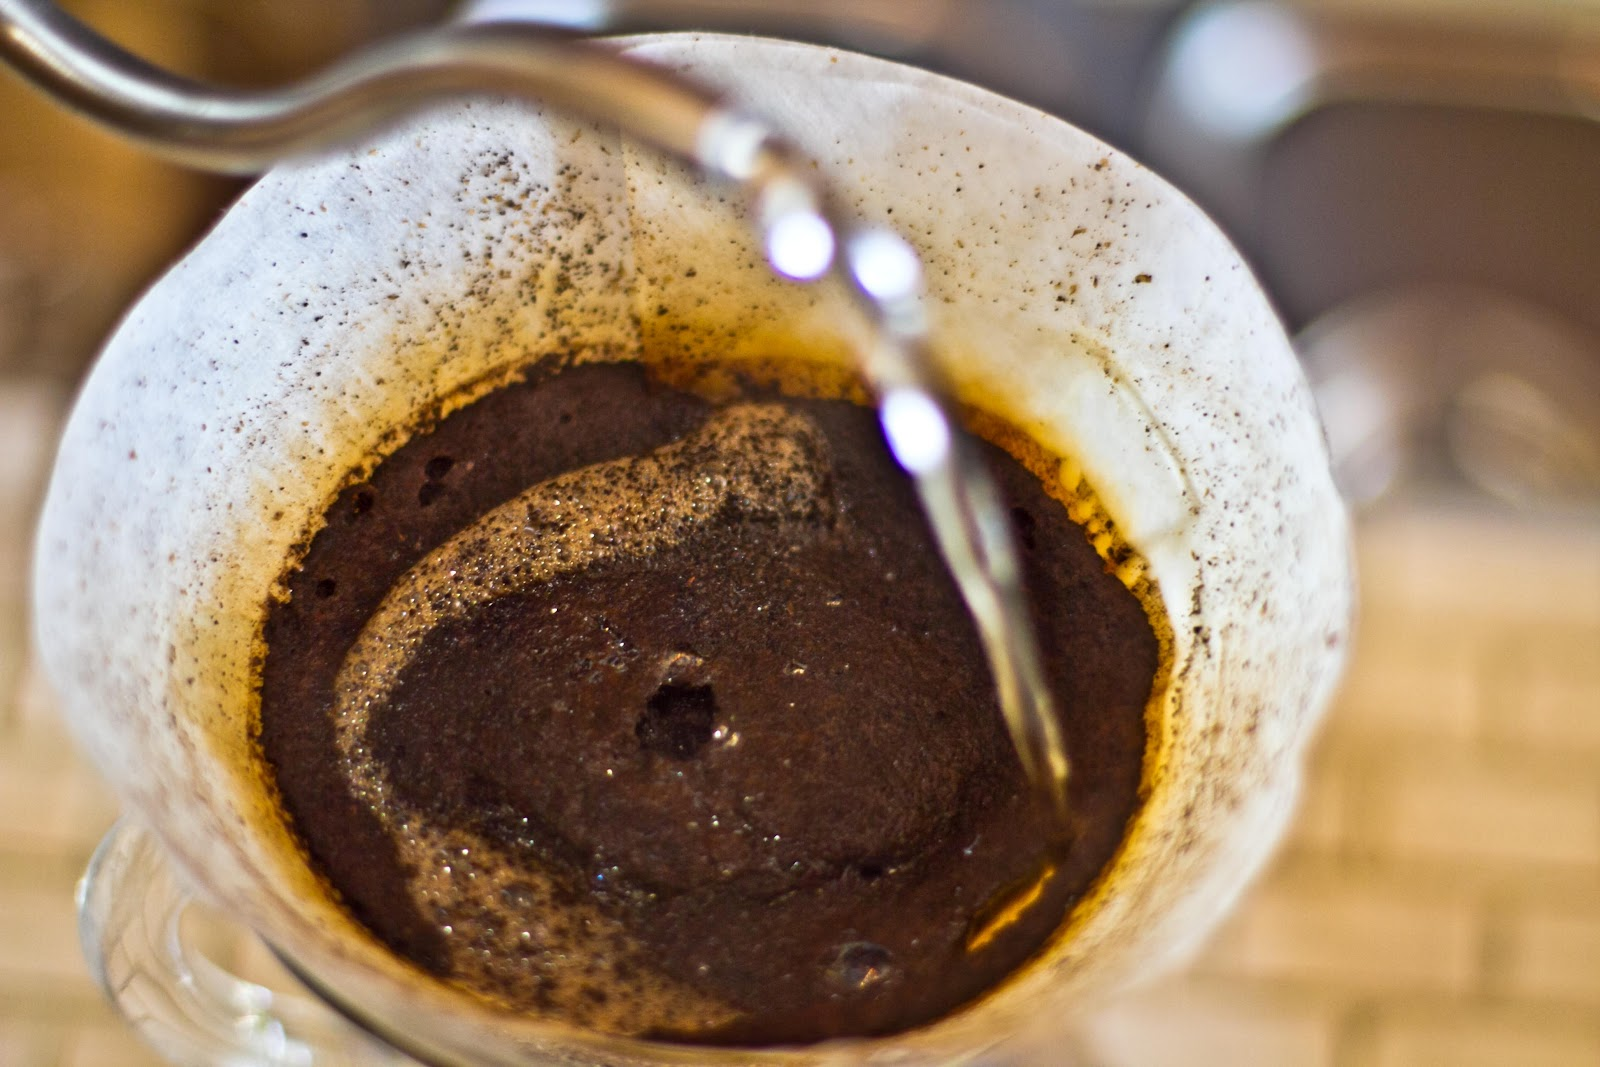
\includegraphics[height=0.25\textwidth]{./figures/chemex-2}
\end{center}
\caption*{The Chemex\tm{} Coffee Maker}
\end{figure}
\clearpage
